\section{Introduction}
In recent years, the Internet of Things (IoT) has been recognized as a major technology that can solve various social problems, and lead the fourth industrial revolution by collaborating with Artificial Intelligence (AI), 5G, and many other things~\cite{ahlgren2016internet}. In addition, varied IoT devices such as home appliances, sensors, actuators, and unmanned vehicles can be connected and interacted with each other through the Internet, and are being used in various fields such as home automation, smart grid, traffic management, and medical aid~\cite{zanella2014internet}. According to the McKinsey's ``The internet of things mapping the value beyond the hype report"~\cite{manyika2015internet}, it is expected that the IoT has a total potential economic impact of \$3.9 trillion to \$11.1 trillion per year in 2025. However, to efficiently use the IoT technologies in the real fields such as smart homes, smart factories, and smart cities, problems that IoT has must be analyzed and addressed.

\subsection{Towards the Internet of Things standards}  
With the development of the IoT industry, various standards for the IoT have been being developed and announced. There are various IoT standards such as oneM2M, Next Generation Standard Interface (NGSI), Open Connectivity Foundation (OCF), Global Standard 1 (GS1). However, IoT services are not using only one standard and these are composed of various standards. In conclusion, in order to support interoperability for platforms and devices developed using various IoT standards, an analysis of the relevant standards is required.

\textbf{oneM2M} is a partnership project of eight national SDOs including Europe, India, Japan, South Korea, and North America to develop global IoT / M2M (Machine-to-machine) common platform standards. oneM2M has been developing a standard technology by targeting a common platform that can be used in various service areas without being dependent on a specific IoT domain. In this context, oneM2M is developing the reference architecture to assist a large number of IoT services such as smart factories, smart cities, smart cars. In terms of the deployment, the oneM2M platform supports useful approaches more than data exchanges for applications. oneM2M platforms provide the interworking features that can allow other IoT platforms or devices to connect to the oneM2M platform. That is, backend systems or external IoT systems can interwork by using an oneM2M standard interworking approach. For example, currently, oneM2M is working with other promising IoT standards such as Open Connectivity Foundation (OCF) and Leightweight Machine to Machine (LwM2M). In addition, beyond integrating with IoT standards, the 3rd Generation Partnership Project (3GPP) is being researched for supporting the interworking feature.

\begin{figure}[H]
	\centering
	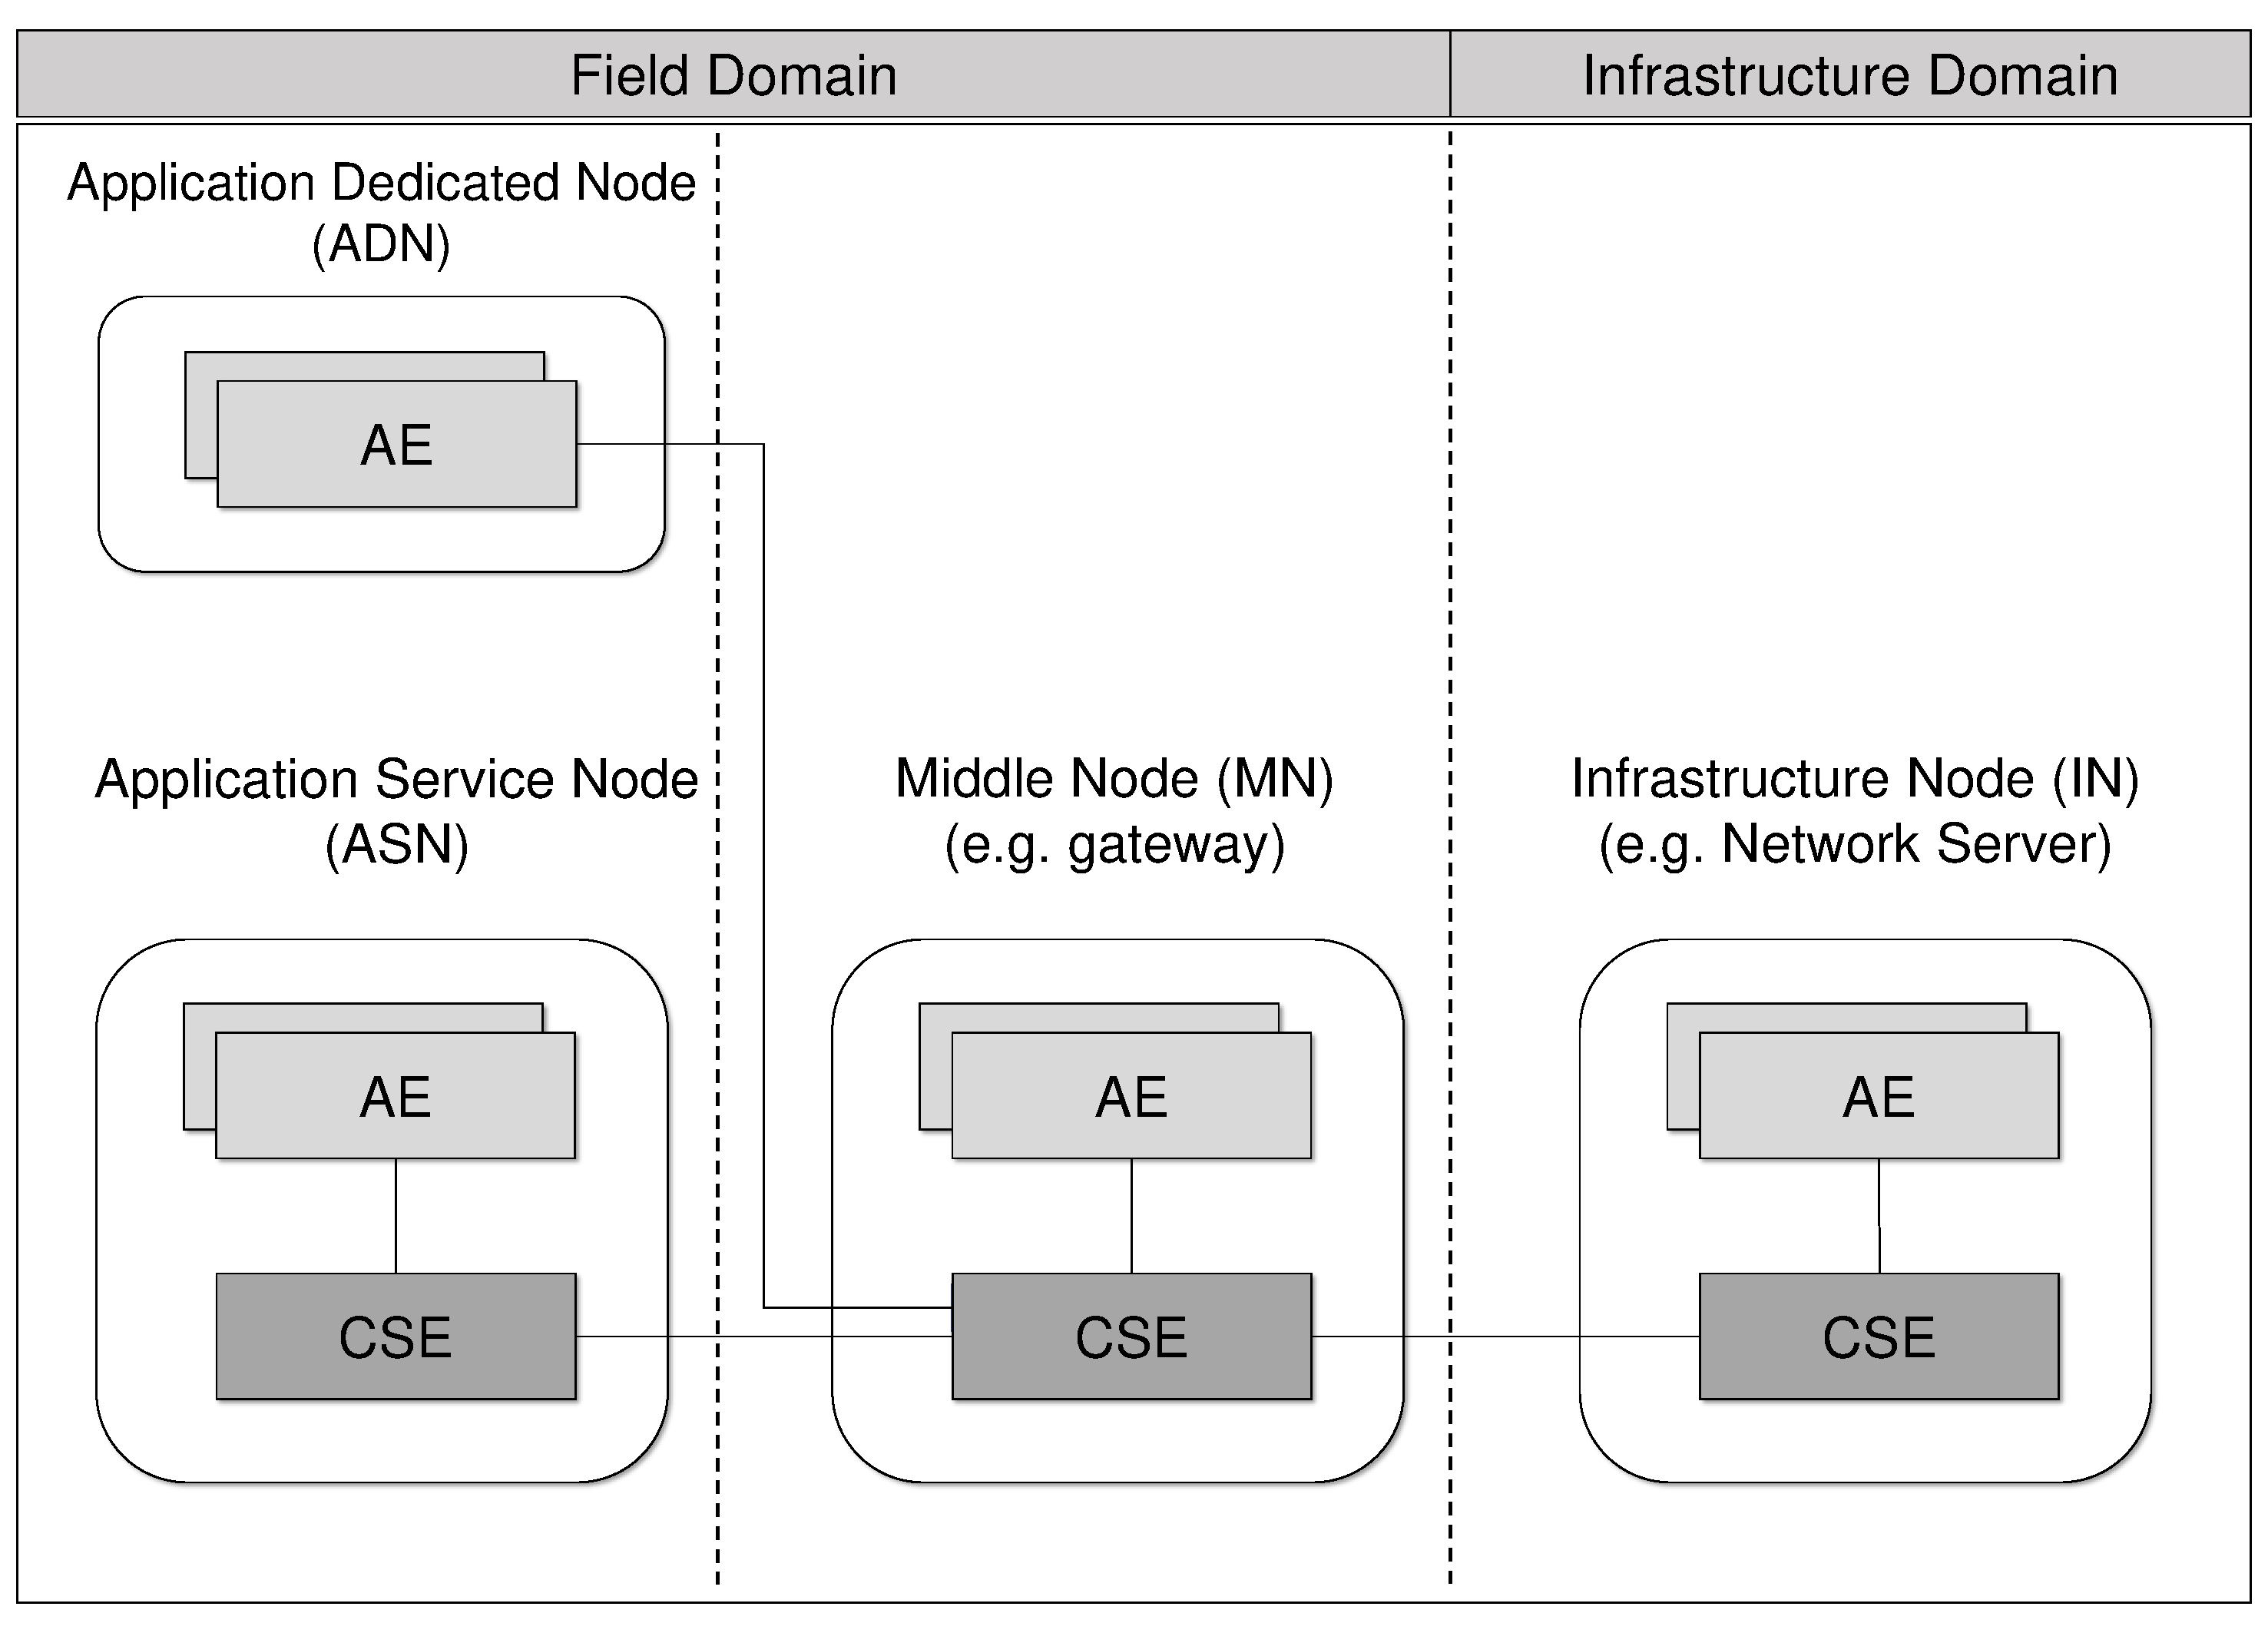
\includegraphics[width=\textwidth]{figures/fig_onem2m_architecture.pdf}
    \caption{oneM2M reference architecture}
    \label{fig:onem2m_reference_architecture}
\end{figure}

To implement the oneM2M IoT systems, four functional entities called nodes are defined and these are described in Fig.~\ref{fig:onem2m_reference_architecture}~\cite{swetina2014toward, husain2014interworking}. Infrastructure Node (IN) represents the IoT server in the reference architecture. IoT gateway can be illustrated as a Middle Node (MN). IoT sensors and actuators are formed in oneM2M environment as an Application Dedicated Node (ADN), Application Service Node (ASN). In addition, oneM2M adopts the Resource Oriented Architecture (ROA) model. that is all IoT devices based on oneM2M standard can be handled as resources based on hierarchical structure~\cite{zhao2018onem2m}, and each resource in the structure has an identifier to classify the resources. In this regard, several resources have been being defined, but, in this dissertation, a fundamental resource to make the IoT services are considered as described in Fig.~\ref{fig:oneM2M_resource_structure}.~\cite{hwang2019interworking}. Common Service Entity (CSE) supports common service functions including registration, discovery, data management. Application Entity (AE) presents the various service logic type. \texttt{<Container>} play a role as data instances. \texttt{<contentInstance>} is storing the real sensored value. \texttt{<CSE>} is a root of all oneM2M child resource, and functional nodes must be comprised of at least one \texttt{<CSE>} or \texttt{<AE>}. The \texttt{<subscription>} resource is created under the resource that \texttt{<subscription>} resource wants to check the status of. The \texttt{<subscription>} has policies for notification and it includes the information of which, when, and how notifications are sent~\cite{2020_onem2m_ts_0001}.

\begin{figure}[H]			% Add figure one
	\centering
	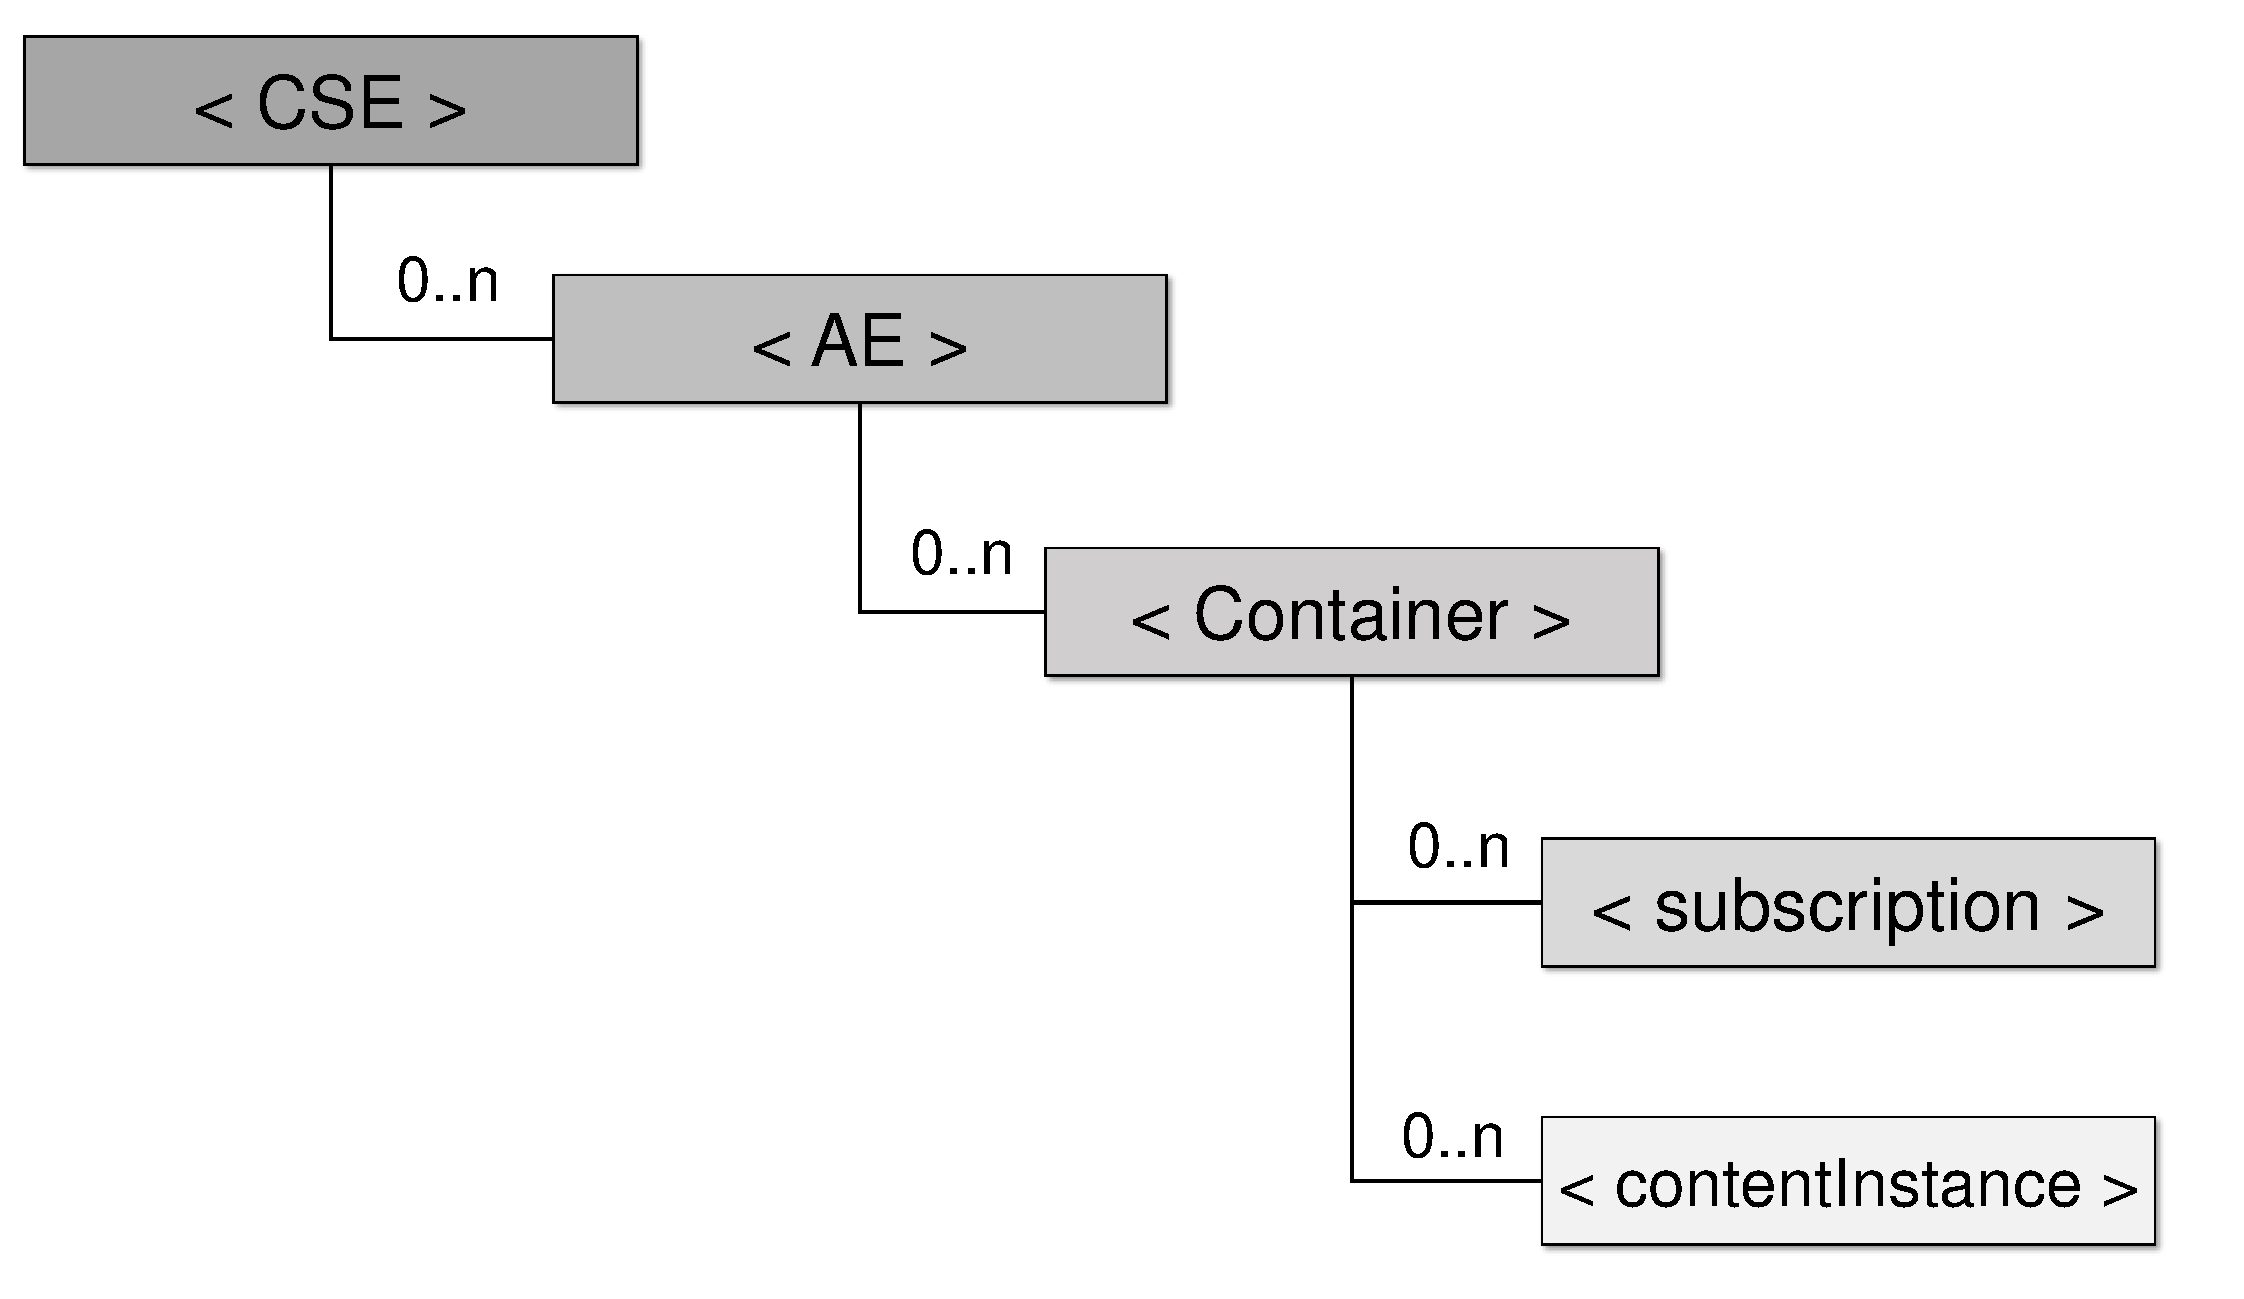
\includegraphics[width=\textwidth]{figures/fig_onem2m_resource_structure.pdf}
    \caption{oneM2M resource structure}
    \label{fig:oneM2M_resource_structure}
\end{figure}

\textbf{FIWARE} is an open cloud-based infrastructure for Future Internet applications and services, consist of different building blocks is called General Enablers (GE) are essentially, reusable software system~\cite{fernandez2016smartport}. Therefore, by integrating several GEs service providers can provide users with FIWARE IoT services such as smart city and smart factory and so on. Currently, based on the FIWARE,  Santander smart city is being operated located in Spain.  In this smart city, it consists of a variety of actuator and sensors can be around 3000 Zigbee devices, 200 devices (mainly mobile) with GPRS communication capabilities, 2000 joint RFID tag/QR code labels deployed both at static locations (streetlights, facades, bus stops) and on-board of mobile vehicles (buses, taxis).

Basically, FIWARE is using Next Generation Service Interface (NGSI) standard. In 2009/2010 Open Mobile Alliance (OMA) specified a set of interfaces called NGSI and defined two interfaces are NGSI-9 (Context Entity Discovery Interface) and NGSI-10 (Context Information Interface)~\cite{bauer2017semantic, kovacs2016standards}. Figure.~\ref{fig:ngsi_datamodel} is showing the example of the data model of NGSI standard. The core concept of NGSI context interfaces is \texttt{Entity}. A lot of physical objects like buildings, rooms, persons can be presented as \texttt{Entity} and these are identified by using Entity identifier and a type. The \texttt{Attribute} is composed of key-value and represents the real value of the \texttt{Entity}. \texttt{Metadata} is additional information of the entity and users can attach their own \texttt{Metadata} to entity's \texttt{Attribute}.

\begin{figure}[H]			% Add figure one
	\centering
	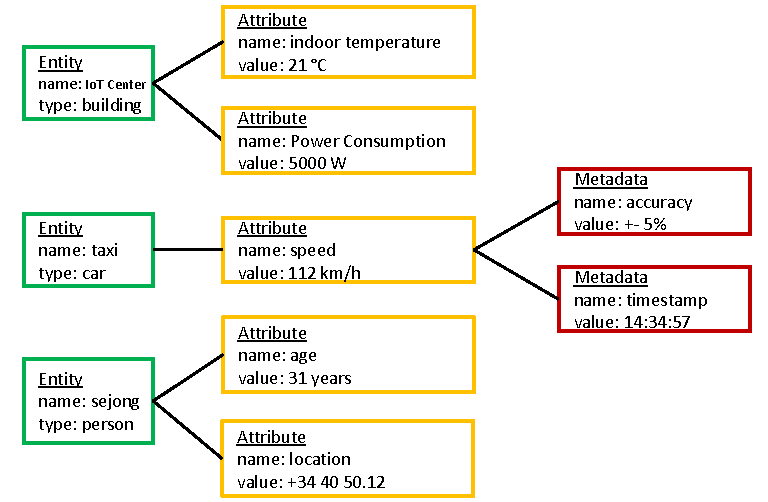
\includegraphics[width=\textwidth]{figures/fig_ngsi_example.pdf}
    \caption{Data model of NGSI}
    \label{fig:ngsi_datamodel}
\end{figure}

Figure.~\ref{fig:ngis_10_api_operation}, \ref{fig:ngis_9_api_operation} presents the operations supported by the NGSI-9 and NGSI-10 interface~\cite{bauer2017wise_iot_d1.3}. Context Management Component (CMC) is defined as an intermediary that manages the context information. In NGSI-10 API operation, Context producers produce context information and context consumers consume context information. Update operation in NGSI-10 allows the actor to update the context value in the CMC. An actor1 can subscribe to be notified from actor2 whenever a certain notification condition occurs.

\begin{figure}[H]			% Add figure one
	\centering
	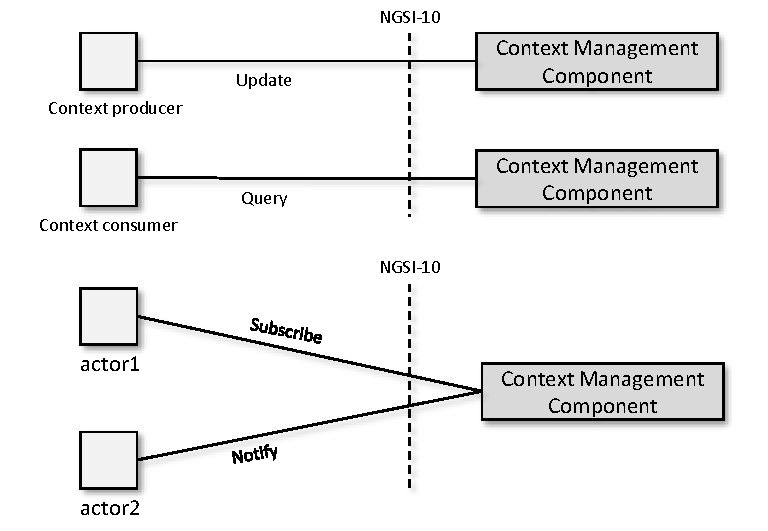
\includegraphics[width=\textwidth]{figures/fig_NGSI_10_api.pdf}
    \caption{NGSI-10 API operations}
    \label{fig:ngis_10_api_operation}
\end{figure}

In the NGSI-9 interface, Actors can register themselves to the CMC, specifying what context information they can give information for, but not include the actual information. Later, the CMC can use this registration information for finding the relevant producers of context information when receiving the requests. In addition, there is a discovery operation that returns currently registered producers, and subscription operations for notifying the availability of the context producers that are eligible for the request.

\begin{figure}[H]			% Add figure one
	\centering
	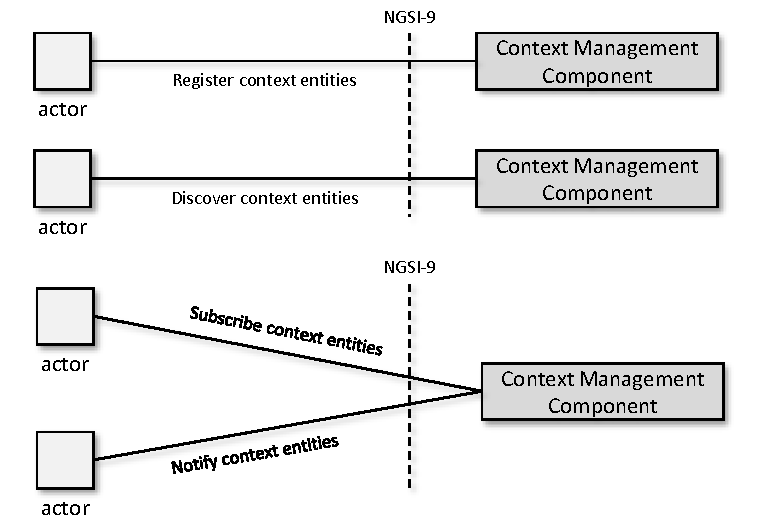
\includegraphics[width=\textwidth]{figures/fig_NGSI_9_api.pdf}
    \caption{NGSI-9 API operations}
    \label{fig:ngis_9_api_operation}
\end{figure}

The FIWARE context broker called Orion is a C++ implementation of the NGSI REST API binding. Orion Context Broker enables users to manage the entire lifecycle of the context information by providing updates, queries, registrations, and subscription operations.  Orion Context Broker allows users to create and manage context elements through updates and queries. In addition, users can also subscribe to context information to be notified when context information changes. It is worth nothing that FIWARE is an opensource detail information can be found here (https://github.com/telefonicaid/fiware-orion).

\begin{figure}[H]			% Add figure one
	\centering
	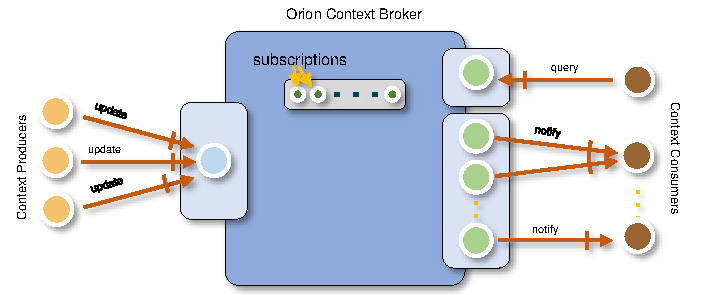
\includegraphics[width=\textwidth]{figures/fig_FIWARE_context_broker.pdf}
    \caption{FIWARE context broker}
    \label{fig:context_broker}
\end{figure}

In standard activity perspective of FIWARE, at present, the Context Information Management (CIM) group which is one of the Industry Specification Group (ISG) under the European Telecommunications Standardization Organization (ETSI) is developing and maintaining the related specifications, and CIM selects the smart cities as the main application domain and it aims at defining the context-based data management API and data platforms. Technically, CIM is developing a context-based API based on FIWARE, which is being developed as a future Internet project in Europe. However, there are differences in the support perspective that CIM supports ontology-based information modeling for semantic integration and JavaScript Object Notation for Linked Data (JSON-LD). The preliminary API specification was released on April 18, and if the CIM standardization result is released continuously, it is expected that the specification for interworking with IoT platform standards such as oneM2M will be established in the future.

\textbf{OCF} is a specification and open source project for delivering the interconnectivity of developers, manufacturers and end-users~\cite{park2017ocf}. There are four founder members including Samsung, Intel, Cisco, and MediaTek, and at present Qualcomm, Microsoft joined OCF as a new member. OCF is providing the open-source project called IoTivity Project and it is being developed based on the OCF specification. In addition, OCF is running on varied software platforms such as Tizen, Android, iOS, Linux.

\textbf{GS1} is an international organization that develops identification and distribution logistics standards using bar code and radio frequency identification (RFID) technology for global supply and demand and logistics chains. Auto-ID Labs, an international joint research institute of the GS1, developed the Open Language for the Internet of Things (Oliot) as an open-source project to develop the GS1 standard.

In addition to the standards described above, ISO/IEC JTC1 WG11, established in October 2015, is developing standards for the smart city ICT reference framework and high-level ontologies for smart cities. In addition, ITU-T formed the ITU-T Focus Group on Smart Sustainable Cities (FG-SSC) and contributed  21 relevant standard documents for activities related to smart city standardization and based on previous research, they have established a new smart city standardization organization called Study Group 20 (SG20). However, such de facto or international standardization organizations have different goals and directions for standardization, and the lack of agreement between standardization organizations raises the issue of IoT interoperability.


\subsection{Problem statements}
This dissertation has conducted preliminary literature research for analyzing what kind of features are essential for successfully constructing the IoT environments. As a result, six candidate features from existing IoT relevant research were gathered. More detailed features' information is described in Table~\ref{tab:smart_city_features} based on literature and these features are as follows: Interoperability, Availability, Scalability, Reliability, Performance, Security.

% Please add the following required packages to your document preamble:
% \usepackage{booktabs}

\def\doitems{\def\item{\par
  \noindent\hbox to 2.3em{\hss\hss}\hangindent=2.3em }}
  
\begin{table}[H]
  \centering
  \renewcommand{\arraystretch}{1.5}
  \tiny
  \begin{tabular}{p{1.39cm}p{1.25cm}p{1.25cm}p{1.25cm}p{1.25cm}p{1.25cm}p{1.25cm}p{1.25cm}}
    \hline
      & \centering Interoperability & \centering Availability & \centering Scailability & \centering Reliability &  \centering Performance & \hspace{0.01cm} Security \\
    \hline
    
     %111111111111111
    \centering Ahlgren, B. et al. \cite{ahlgren2016internet} &
    \doitems   
        \item O & 
    \doitems   
        \item O &
    \doitems   
        \item O &
    \doitems   
        \item -- &
    \doitems   
        \item -- &
    \doitems   
        \item -- \\
    \hline

    \centering Gluhak, Alexander, et al.\cite{gluhak2011survey} & 
    \doitems   
        \item O & 
    \doitems   
        \item -- &
    \doitems   
        \item O &
    \doitems   
        \item -- &
    \doitems   
        \item -- &
    \doitems   
        \item -- \\
    \hline
    
	%111111111111111
    \centering Yun et al. \cite{yun2016interworking} & 
    \doitems   
        \item O & 
    \doitems   
        \item O &
    \doitems   
        \item O &
    \doitems   
        \item -- &
    \doitems   
        \item -- &
    \doitems   
        \item -- \\
    \hline
    
    \centering Sarkar, Chayan, et al. \cite{sarkar2014scalable} & 
    \doitems   
        \item O & 
    \doitems   
        \item O &
    \doitems   
        \item -- &
    \doitems   
        \item -- &
    \doitems   
        \item -- &
    \doitems   
        \item -- \\
    \hline
    
    \centering R Roman et al. \cite{roman2013features} & 
    \doitems   
        \item O & 
    \doitems   
        \item -- &
    \doitems   
        \item -- &
    \doitems   
        \item O &
    \doitems   
        \item -- &
    \doitems   
        \item O \\
    \hline
    
    \centering H Arasteh et al. \cite{arasteh2016iot} & 
    \doitems   
        \item O & 
    \doitems   
        \item -- &
    \doitems   
        \item O &
    \doitems   
        \item O &
    \doitems   
        \item -- &
    \doitems   
        \item O \\
    \hline
    
    \centering Al-Fuqaha, Ala, et al. \cite{al2015internet} & 
    \doitems   
        \item O & 
    \doitems   
        \item O &
    \doitems   
        \item O &
    \doitems   
        \item O &
    \doitems   
        \item O &
    \doitems   
        \item O \\
    \hline
    
    \centering Mehmood, Yasir, et al. \cite{mehmood2017internet} & 
    \doitems   
        \item O & 
    \doitems   
        \item O &
    \doitems   
        \item O &
    \doitems   
        \item -- &
    \doitems   
        \item -- &
    \doitems   
        \item O \\
    \hline
    
    \centering Wenge, Rong, et al. \cite{wenge2014smart} & 
    \doitems   
        \item O & 
    \doitems   
        \item -- &
    \doitems   
        \item -- &
    \doitems   
        \item -- &
    \doitems   
        \item -- &
    \doitems   
        \item O \\
    \hline
  \end{tabular}
  \caption{Main features for the IoT environments}
    \label{tab:smart_city_features}
\end{table}

\begin{itemize}
    \item \textbf{Interoperaiblity:} End-to-End interoperability is a challenge for the smart cities interworking due to the need to handle a large number of heterogeneous things that belong to different platforms.

    \item \textbf{Availability:} Availability of the smart city services must be realized to provide anywhere and anytime services for citizens even users are moving different smart cities.

    \item \textbf{Scalability:} The scalability of the smart cities refers to the ability to add new IoT enabled smart cities, services and functions for customers without negatively affecting the quality of existing services.

    \item \textbf{Reliability:} Reliability ensures the proper working of the system in terms of its specification. Reliability's aim is to increase the success probability of IoT service delivery.

    \item \textbf{Performance:} The IoT devices need to be evaluated to provide the best possible performance. Smart cities must not make performance degradation of smart city services.

    %\item \textbf{Federation:} Federation with other smart cities is necessary to achieve scale or add capabilities for experimentation that are not locally available.
 
    \item \textbf{Security} Since the data in a smart city includes individual, enterprise, and state economic data, providing the right level of security for sensitive information between smart cities is an important feature.
\end{itemize}

As shown in Table~\ref{tab:smart_city_features}, the \textbf{\texttt{interoperability}} problem is pointed out as a problem to be solved first. More specifically, since most IoT platforms developed so far provide IoT services using the platform manufacturers' own standards and data models, there is a problem that compatibility with other platforms is not guaranteed~\cite{nist2017internet, aft2016interoperability}. If interoperability is not guaranteed, IoT platforms cannot interoperate with or exchange data with things developed according to different standards, and cause technical and economic problems such as delays in the introduction of large-scale IoT technology and increased operating costs. In addition, McKinsey's `` 2015 THE INTERNET OF THINGS MAPPING THE VALUE BEYOND THE HYPE '' report~\cite{manyika2015internet} showed that the IoT platform should be supported for interoperability in order to achieve additional economic effects of more than 4 trillion dollars annually. Since most IoT platforms currently being deployed in various industry fields are not built using a single unified IoT standard, so they cannot interoperate with each other. Therefore, the cost of replacing an already deployed system can be substantial to support other IoT standards. For example, in such an environment, in order to deliver IoT services developed in Europe, new services must be developed in South Korea.

With regard to the IoT standard testing, for assuring the interoperability of IoT services, conformance and interoperability testing are highly important to ensure that independent implementation based on the same or different standard are interoperable~\cite{kim2017towards}. Furthermore, IoT services are pervasive in people's lives and impact on every industry area. Therefore, providing a sustainable and stable quality of IoT services is essential and to avoid fatal risks caused by the dysfunctional devices or not working products with others~\cite{brady2017towards}. Therefore, testing a huge amount of IoT devices and platforms in real-time is becoming one of the most important parts of IoT technologies~\cite{ahmed2019aspects, sand2015iot}. To conclude, it is important for the IoT services to deploy interoperable and reliable IoT platforms or IoT devices. Therefore, adequate IoT testing approaches are needed to support interoperable and reliable IoT environments. However, as challenges for IoT application testing, most of the studies regarding IoT testing do not discuss standard-based IoT testing. In addition, regarding the testing intervention by a human, in the situation of the traditional IoT testing, the problem is that the human manually tests the IoT applications. It is impossible to test a lot of applications manually and human intervention can make side effects on the testing results. Therefore, the sure-fireway is that it makes the testing procedures automated.

\subsection{Contributions}
In this dissertation, mainly two research areas are studied for IoT environments. First, to solve the IoT standard interoperability issues, three interworking models are proposed. To interconnect the existing IoT-based services without modification or changes existing systems, by referencing the interworking models proposed in this dissertation, IoT service developers could get insight regarding the IoT standard interworking. In addition, because an evaluation matrix of the pros and cons of the three interworking models is included, according to the requirements of the IoT services, developers also can make a good selection for the desirable IWMs. For proving the above contributions, as a practical example, IWMs are explained based on the smart city scenario.

Regarding the IoT conformance testing approaches, the fully-automated testing approach is studied and described in this dissertation. In detail, standard-based triggering messages and automated testing procedures are newly developed. As a result, this approach fully automates testing procedures for IoT applications; therefore, many IoT applications can be easily tested without human intervention. In addition, together with an experimental evaluation, triggering-based IoT testing mechanisms show the advantage in terms of performance and testing time. Finally, the proposed triggering mechanism is reflected in one of the normative specifications as a standard-based testing mechanism in oneM2M IoT standard. Therefore, the triggering IoT testing feature based on the proposed approach in oneM2M has already been included in designated oneM2M testing tools. In this context, the automated testing approach contributes to the rapid propagation of IoT standards by reducing the time required of the testing and certification process for the testing certification body. Additionally, by empirical analyzing existing IoT testing-related projects, a conceptual architecture of the IoT testing framework that can increase the reliability of the three interworking models presented above is proposed as a future work.

\subsection{Dissertation outline}
This dissertation is mainly organized as follows. The section~\ref{sec:smartcity_interworking} describes why interworking among IoT systems is needed by exemplifying the scenario based on smart cities and three interworking models are included as a solution for this issue. The section~\ref{sec:smartcity_testing} illustrates an automated IoT testing mechanism for enhancing the traditional testing approach when conducting IoT application testing. Finally, the last section concludes this dissertation and proposes the future work.

\clearpage